\section{Technische Grundlagen}
\label{sec:techngrund}

In der folgenden Sektion wird auf das Wissen eingenangen, welches benötigt wurde um das System zu implementieren. 

\subsection{Fahrzeugtechnik}
Das Entwicklungsteam des Projekts stammt aus der Abteilung für Informationstechnologie des TGMs, daher hatten wir die benötigten Grundkenntnisse von Fahrzeugtechnik nicht. Im Verlauf des Projekts wurde durch die Hilfe von Prof. Dipl.-Ing. Heinz Neuburger eine Implementierung entwickelt, mit welcher die benötigten Sensordaten aus dem Auto verwendbar gemacht worden sind.
\lfoot{Autor: Raphael Simsek}
\subsubsection{OBD II}
\label{subsec:obd2}

\paragraph{Definition}
Häufig ist die OBD-II Schnittstelle bei Autofahrern für das Auslösen von Problemen bekannt. Genannte Probleme stammen vielfach von \textit{Error-Codes oder Diagnostic Trouble Codes (DTCs)}, welche aus der \textit{Engine Control Unit} (siehe xy Kapitel) ausgeworfen werden und häufig das komplette Vehikel unfreiwillig stilllegen. Derartige DTCs müssen folglich in einer Fachwerkstatt reseted werden. Die ECU ist ... (referenzieren). \todo{add content concerning ECU} Weitere Informationen zum Hintergrund des System sind unter Auslesen in diesem Kapitel auffindbar. 
Die OBD-II Schnittstelle ist eine standardisierte Schnittstelle. Die Schnittstelle verschafft Zugriff auf Daten des Motormanagements. Für die Auslesung der Daten des Motormanagments ( \textit{Engine Control Unit}) ist ein passendes Auslesegerät nötig. Sie hat unterschiedliche Versionen, welche auf die verschiedenen Kontinente aufgeschlüsselt wurden. Die Schnittstelle wird vor allem für das Auslesen vom Fehlercodes aus dem Motormanagement verwendet. Sie kann aber zusätzlich dazu auch durch standardisierte Datenabfragen (Mode 01) Echtzeit Daten liefern.

\paragraph{Standardisierung}
Timeline:
\begin{itemize}
	\item 1980: General Motors führt \textit{assembly line diagnostic link (ALDL)} ein
	\item 1988: Die \textit{Society of Automotive Engineers (SAE)} rät einen standardisierten Konnektor mit Testsignalen an
	\item 1991: \textit{California Air Resources Board (CARB)} fordert, dass alle Autos die ab 1991 in Kalifornien verkauft werden, Basisfunktionalität mit OBD aufweisen
	\item 1996: Die OBD-II Spezifikation wird für alle Autos die in den USA verkauft werden Pflicht
	\item 2001: EOBD wird obligatorisch für Benzin-Fahrzeuge innerhalb der EU
	\item 2003: EOBD wird obligatorisch für Diesel-Fahrzeuge innerhalb der EU
\end{itemize}
\cite{SIMR.CH2-obd2.Timeline}
Die OBD-II Schnittstelle wurde zuerst in den USA etabliert, wo sie auch 1996 zuerst verpflichtend wurde. Zusätzlich wurde EOBD als Standard definiert, womit die europäische Umsetzung des OBD-II Standards beschrieben wird \cite{SIMR.CH2-obd2.EUP-D98/69/EC}. Der wesentliche Unterschied ist die Standardisierung. Die ist zwar technisch zwischen SAE J1962 und ISO/DIS 15031 equivalent, es wurden aber trotzdem unterschiedliche Namen gewählt \cite{SIMR.CH2-obd2.SAEJ1962}. Ferner gibt es einen australischen \cite{SIMR.CH2-obd2.AU-MVSA1989} und eine japanischen Standard.

\paragraph{Charakterisierung}
Außerdem wurde innerhalb der Standardisierung die Form des Konnektors festgelegt. Dieser ist entweder als OBD-II A oder B Konnektor definiert. Der A Konnektor ist für alle Fahrzeuge mit 12 V Bordspannung und hat die Form eines D mit einer Nut in der Mitte, um die Pins zu behausen. Der B Konnektor verwendet ebenfalls die Form eines D's, allerdings ist dieser Konnektor für Fahrzeuge mit 24V Bordspannung. Diese sind beispielsweise Lastkraftfahrzeuge. Bei diesem Konnektor ist die Nut in der Mitte unterbrochen, um es unmöglich zu machen einen männlichen Konnektor des A-Typs einzustecken. Dieser Konnektor könnte nämlich aufgrund von Überspannung zu einem Defekt führen. Es ist also der B Konnektor sowohl mit A und B kompatibel, allerdings ist der A Konnektor nur mit seinesgleichen verwendbar.

\begin{figure}[!htb]\centering
   \begin{minipage}{0.49\textwidth}
     \frame{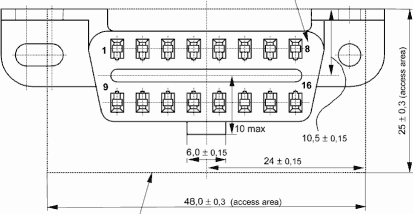
\includegraphics[width=\linewidth]{images/j1962f_type_a}}
     \caption{Typ A, OBD II Konnektor \cite{SIMR.CH2-obd2.OBDIITypeA}}\label{Fig:Data1}
   \end{minipage}
   \begin {minipage}{0.49\textwidth}
     \frame{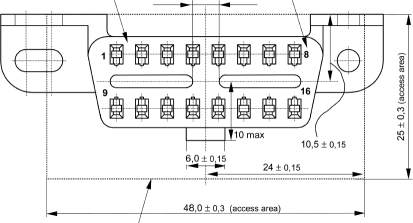
\includegraphics[width=\linewidth]{images/j1962f_type_b}}
     \caption{Typ B, OBD II Konnektor \cite{SIMR.CH2-obd2.OBDIITypeB}}\label{Fig:Data2}
   \end{minipage}
\end{figure}


\paragraph{Positionierung / Lokalisierung\nextline}
Die OBD II Schnittstelle muss innerhalb der EU bei allen PKW mit Benzinmotor ab 2001 und bei allen PKW mit Dieselmotor ab 2004 vom Fahrer erreichbar verbaut sein. Aus diesem Grund wird die OBD II Schnittstelle von gängigen Automobilherstellern oft fahrerseitig im Bereich der Pedale, im Bereich der Mittelkonsole oder links neben dem Lenkrad montiert. Die Schnittstelle wird häufig in  Bereich der Fahrzeugsicherungen angebracht (z.B. bei vielen Modellen der Marke VW).
Exemplarisch können Sie hier die Lokalisierung der OBD II Schnittstelle an einem Golf VI erkennen. Diese Schnittstelle ist hier unterhalb einer ohne Werkzeug entfernbaren Abdeckung versteckt. Wie auf dem Foto erkennbar ist die Schnittstelle hier im Fußraum der Fahrerseite, links der Pedale platziert.

\begin{figure}[!htb]\centering
	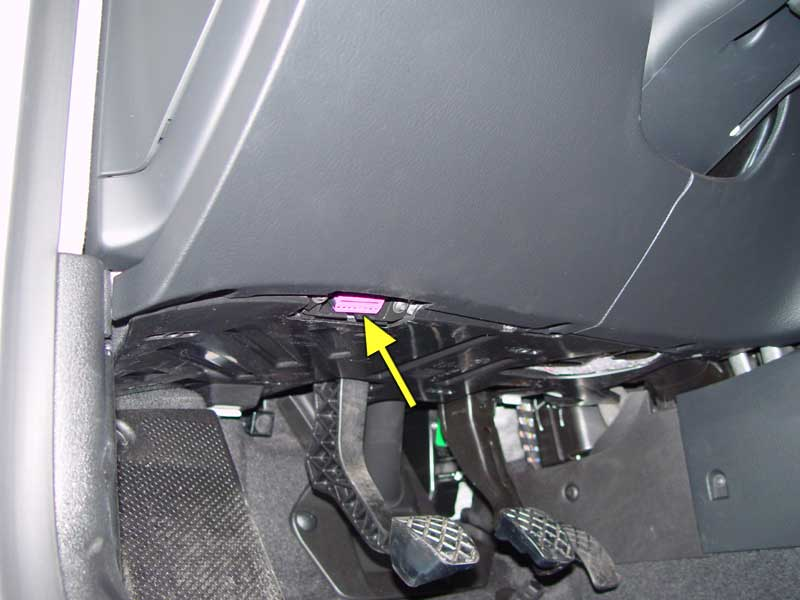
\includegraphics[width=0.5\textwidth]{images/golfobd}
	\caption{OBD II Konnektor bei einem Golf VI \cite{SIMR.CH2-obd2.GolfOBD}}\label{Fig:Data3}
\end{figure}

Bei einem BMW 3er E90 ist der OBD Konnektor hinter der linken Fußraumverkleidung der Fahrerseite zu finden. Er wurde unter einer kleinen Abdeckung, welche mit \"OBD\" beschriftet ist, verdeckt. Die OBD Schnittstelle ist hier vertikal angeordnet.

\begin{figure}[!htb]\centering
	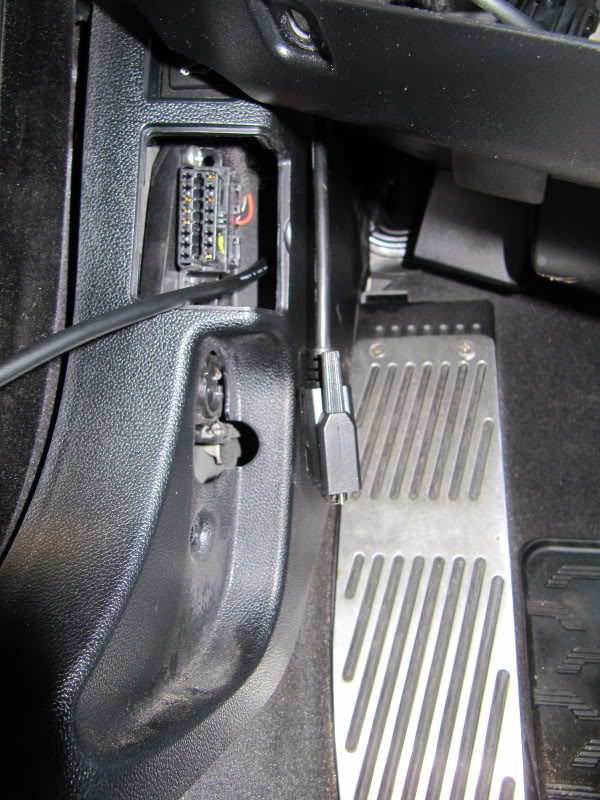
\includegraphics[width=0.6\textwidth]{images/3erobd}
	\caption{OBD II Konnektor bei einem BMW 3er E90 \cite{SIMR.CH2-obd2.3erOBD}}\label{Fig:Data3}
\end{figure}

\paragraph{Auslesen}
Das bei der OBD-II Schnittstelle verwendete Datenübertragungsprotokoll basiert auf einem \textit{Controller Area Network (CAN)}-Bus. Dies das Auslesen mit diesem Bus erfolgt in der Regel so:
\begin{itemize}
	\item Der Mechaniker schließt ein Auslesegerät an die OBD-II Schnittstelle des Fahrzeugs an
	\item Der Mechaniker gibt die gewollte PID ein
	\item Das Auslesegerät schickt die Anfrage an den Bus des Fahrzeugs (Protokolle: CAN, VPW, PWM, ISO, KWP vor 2008; nach 2008 ausschließlich CAN)
	\item Ein Gerät innerhalb des Bus erkennt dann dass es für den PID zuständig ist, der abgefragt wurde und liefert den Wert der PID an den Bus
	\item Das Auslesegerät ließt die Antwort aus und zeigt sie dem Mechaniker, welcher dann entscheidet welche weiteren Schritte nötig sind
\end{itemize} \todo{Add text describing the CAN BUS protocol \url{http://www.me-systeme.de/canbus.html\#1578569eb20a3da0f}, if still needed}

Die OBD-II Schnittstelle muss laut Norm zur Verfügung stellen, welche Daten die Schnittstelle ausgeben kann und welche Standards (siehe am Beginn des Kapitels) die Schnittstelle unterstützt \cite{SIMR.CH2-obd2.PIDMustHave}. Diese werden über standardisierte Kennnummern, sogenannte PID (Parameter IDentification). Da Fahrzeughersteller fast immer noch zusätzliche Daten bereitstellen, können alle unterstützten PIDs ausgelesen werden. Vorgehensweise mittels des verwendeten Bluetooth ELM 327 Dongles: 

\begin{enumerate}
	\item Verbindung aufbauen
	\begin{enumerate}
		\item Verbindung mit Bluetooth OBD-II ELM327 Chip aufbauen
		\item Verbindung zum seriellen COM-Port aufbauen 
	\end{enumerate}
	\item Mode \# + PID \# (zusammen also 0100/0120/0140/0160/0180/...) abfragen
	\item Zurückgegebene 4 Byte von Hexadezimal zu Binär umrechnen
	\item In eine Tabelle einfügen und überprüfen welche PID's unterstützt sind
\end{enumerate}

Jedes Bit entspricht einer unterstützten PID. In Tabelle 1 wird ein typisches Ergebnis einer PID-Abfrage „BE1FA813“ gezeigt.

\begin{table}[!htb]
\centering
\resizebox{\columnwidth}{!}{%
\begin{tabular}{|l|c|c|c|c|c|c|c|c|c|c|c|c|c|c|c|c|}
\hline
Hexadecimal & \multicolumn{4}{c|}{B} & \multicolumn{4}{c|}{E} & \multicolumn{4}{c|}{1} & \multicolumn{4}{c|}{F} \\ \hline
Binary & 1 & 0 & 1 & 1 & 1 & 1 & 1 & 0 & 0 & 0 & 0 & 1 & 1 & 1 & 1 & 1 \\ \hline
Supported? & \cellcolor[HTML]{9AFF99}Yes & \cellcolor[HTML]{FD6864}No & \cellcolor[HTML]{9AFF99}Yes & \cellcolor[HTML]{9AFF99}Yes & \cellcolor[HTML]{9AFF99}Yes & \cellcolor[HTML]{9AFF99}Yes & \cellcolor[HTML]{9AFF99}Yes & \cellcolor[HTML]{FD6864}No & \cellcolor[HTML]{FD6864}No & \cellcolor[HTML]{FD6864}No & \cellcolor[HTML]{FD6864}No & \cellcolor[HTML]{9AFF99}Yes & \cellcolor[HTML]{9AFF99}Yes & \cellcolor[HTML]{9AFF99}Yes & \cellcolor[HTML]{9AFF99}Yes & \cellcolor[HTML]{9AFF99}Yes \\ \hline
PID number & 1 & 2 & 3 & 4 & 5 & 6 & 7 & 8 & 9 & 0A & 0B & 0C & 0D & 0E & 0F & 10 \\ \hline
Hexadecimal & \multicolumn{4}{c|}{A} & \multicolumn{4}{c|}{8} & \multicolumn{4}{c|}{1} & \multicolumn{4}{c|}{3} \\ \hline
Binary & 1 & 0 & 1 & 0 & 1 & 0 & 0 & 0 & 0 & 0 & 0 & 1 & 0 & 0 & 1 & 1 \\ \hline
Supported? & \cellcolor[HTML]{9AFF99}Yes & \cellcolor[HTML]{FD6864}No & \cellcolor[HTML]{9AFF99}Yes & \cellcolor[HTML]{FD6864}No & \cellcolor[HTML]{9AFF99}Yes & \cellcolor[HTML]{FD6864}No & \cellcolor[HTML]{FD6864}No & \cellcolor[HTML]{FD6864}No & \cellcolor[HTML]{FD6864}No & \cellcolor[HTML]{FD6864}No & \cellcolor[HTML]{FD6864}No & \cellcolor[HTML]{9AFF99}Yes & \cellcolor[HTML]{FD6864}No & \cellcolor[HTML]{FD6864}No & \cellcolor[HTML]{9AFF99}Yes & \cellcolor[HTML]{9AFF99}Yes \\ \hline
PID number & 11 & 12 & 13 & 14 & 15 & 16 & 17 & 18 & 19 & 1A & 1B & 1C & 1D & 1E & 1F & 20 \\ \hline
\end{tabular}
}
\caption{Tabelle zur bitweisen Verarbeitung der Hexadezimal Zeichenkette \cite{SIMR.CH2-obd2.HextoBinary}}
\label{tableHextoPID}
\end{table}

Es wurden innerhalb des Projektes ausschließlich Daten des PID Mode 01 (Realtime Data) verwendet. Grundsätzlich sind alle Mode 01 PIDs zwischen 00 und 87 bezüglich ihrer Einheiten und Bereiche standardisiert. Die PIDs zwischen A0 und E0 sind komplett frei für Autohersteller verfügbar um abseits der Norm eigene Daten einzupflegen. 

Während des Projektes wurden die PIDs 04 - Calculated engine load [\%] und 0C - Rotations per Minute [0-16.383,75] für den Schaltvorschlag verwendet, wozu im nächsten Abschnitt genauere Informationen gefunden werden können. Für die Errechnung des \ce{CO2}-Ausstoßes wurde PID 43 - absolute load value [0-25.700] und 5E - engine fuel rate [L/h] eingesetzt.
\todo{Add PID's and what they are being used for}
\clearpage % DO NOT REMOVE
\lfoot{Autor: Raphael Simek}
\subsubsection{Motorwirkungsgrad}
\label{subsec:motorwirkungsgrad}

\textbf{Einführung\newline}
Grundsätzlich wurde sich mit dem Motorwirkungsgrad beschäftigt, um feststellen zu können, welcher Schaltpunkt möglichst effizient bezüglich des Motorwirkungsgrads ist. Denn es gibt nicht einen einzigen Wirkungsgrad, sondern ein niedriger Spritverbrauch (Motorwirkungsgrad) heißt auch nicht gleichzeitig ein niedriger \ce{CO2}-Ausstoß, denn der Katalysator hat erneut seinen eigenen Wirkungsgrad, welcher für diese Rechnung einbezogen wurde. Für das Diplomprojekt wurde sich aber auf den Motorwirkungsgrad fokussiert.

\textbf{heutige Probleme durch die Öl-Förderung\newline}
\begin{wrapfigure}{r}{0.6\textwidth}\centering
    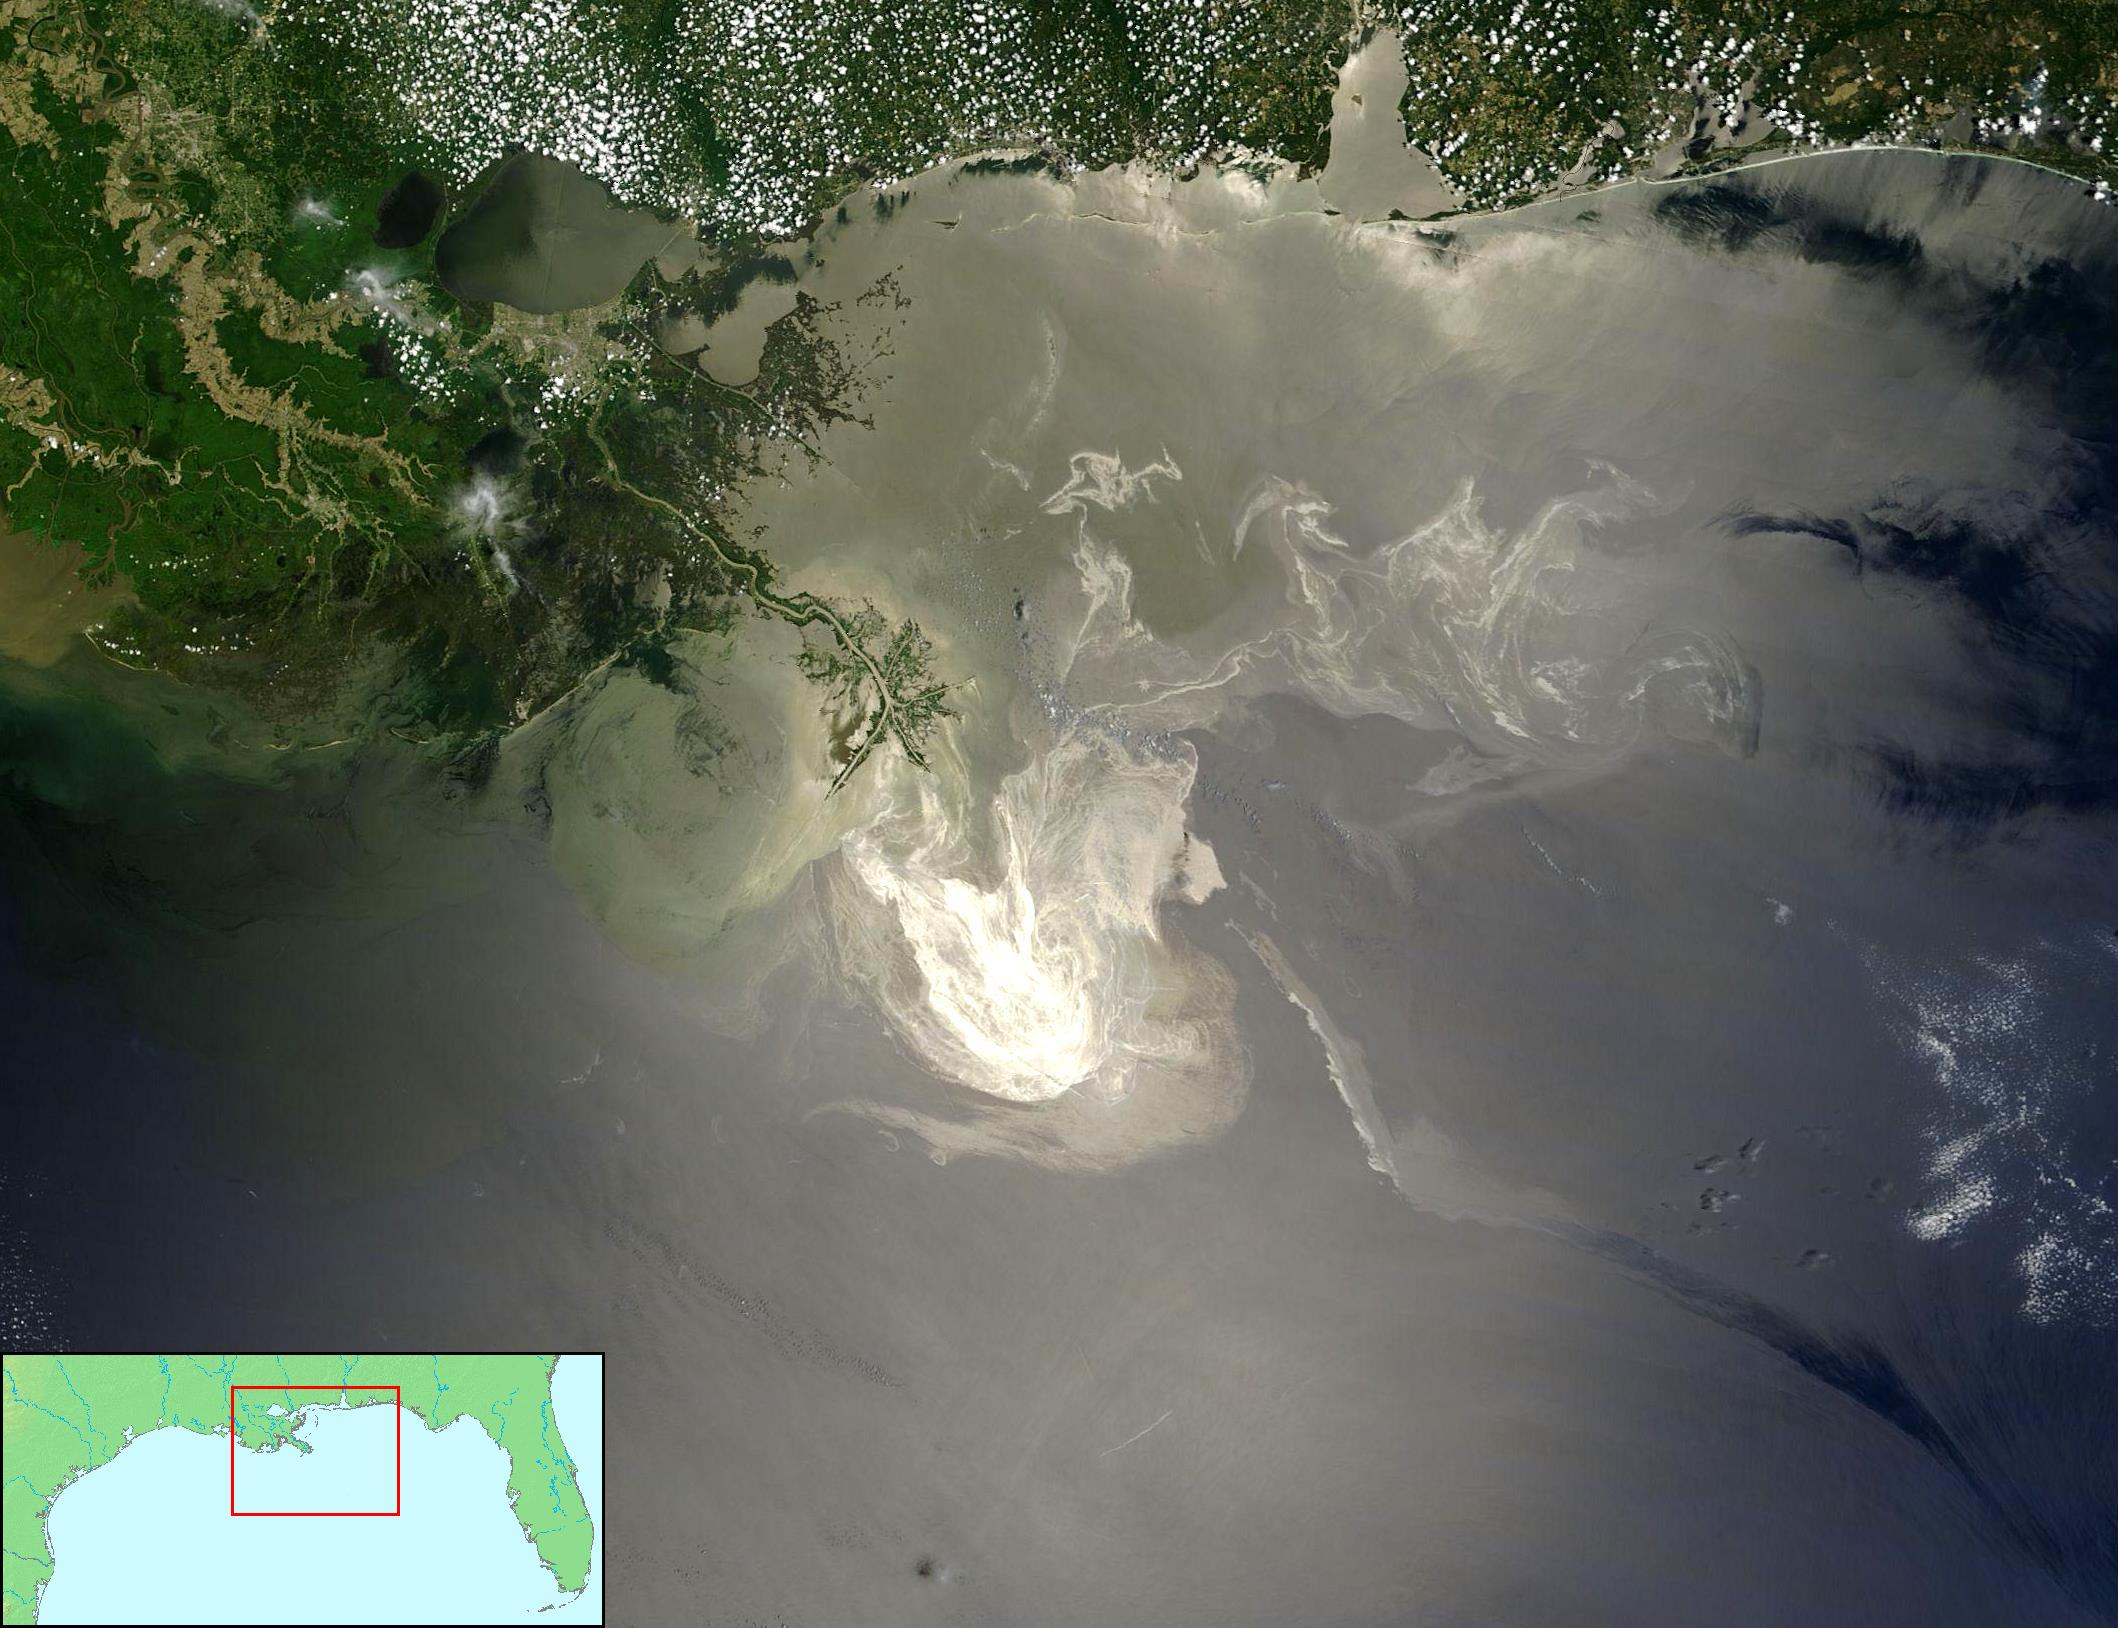
\includegraphics[width=0.6\textwidth]{images/bpOilSpillSatelite}
    \caption{1 Monat nach der Explosion \cite{SIMR.CH2-motorwirkungsgrad.bpOilSpillSatelite}} \label{Fig:imgBPOilSpill}
\end{wrapfigure}
Dieses Thema ist besonders im Bezug auf die immer restriktiveren Emissionsbestimmungen und die häufig hohen Kraftstoffpreise von Interesse für Autofahrer. Zusätzlich sind fossile Brennstoffe, bekanntlich, nicht erneuerbare Ressourcen, weshalb die Vorkommen zeitnah erschöpft sein werden. Genau deshalb ist es besonders wichtig sparsam und ökonomisch mit der bald erschöpften Ressource Erdöl umzugehen. 
Denn die Öl-Förderung erzeugt schon heute Naturkatastrophen und Umweltverschmutzung und wird immer schwerer zu erlangen.
Naturkatastrophen wie BP's \textit{Deepwater Horizon} Ölpest aus dem Jahre 2010 \cite{SIMR.CH2-motorwirkungsgrad.BPSpillGeneral}, bei welcher 3 Jahre nach der Explosion weiterhin Rekordzahlen von Delphinen und Wasserschildkröten starben \cite{SIMR.CH2-motorwirkungsgrad.BPSpillDeaths}. 

Die Probleme, die durch die Öl-Förderung entstehen enden aber noch nicht hier, denn Öl wird auch immer schwerer zu erreichen. Deshalb müssen Techniken wie Fracking eingesetzt werden, um die letzen Öl-Reserven zwischen den Bohrungen zu fördern, wofür ein Cocktail von für Menschen giftige und sogar radioaktive Chemikalien verwendet werden \cite{SIMR.CH2-motorwirkungsgrad.FrackingChemicals}. Es wird geschätzt dass 30-70\% dieses Cocktails wieder an die Oberfläche kommen wird und das Grundwasser verseuchen wird \cite{SIMR.CH2-motorwirkungsgrad.FrackingGroundwater}.

\begin{figure}[!htb]\centering
	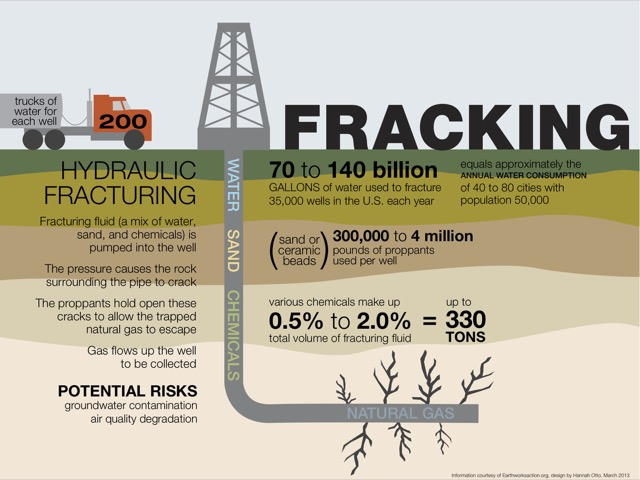
\includegraphics[width=0.6\textwidth]{images/frackingInfographic}
	\caption{Fracking in einem Bild erklärt \cite{SIMR.CH2-motorwirkungsgrad.frackingDescription}}\label{Fig:imgFrackingDesc}
\end{figure}

\newpage
\textbf{zukünftige Probleme durch Öl-Förderung\nextline}
All diese, bereits vorkommenden, Probleme scheinen aber in keinem Verhältnis zu den Problemen die uns erwarten, wenn wir alles Öl auf der Erde verbrauchen, zu stehen. Sollten wir nämlich alles Öl auf der Erde verbrennen, so würde uns ein Anstieg des Ozeans um 44ft (13.41m) erwarten. \cite{SIMR.CH2-motorwirkungsgrad.SeaLevelRiseAllOilBurnt} Da dies aber unwahrscheinlich zeitnah passieren wird, wurde auch ein Anstieg von 4ft (0.91m) innerhalb eines Jahrhunderts, bei anhaltendem Ölverbrauch, von der NASA vorhergesagt. \cite{SIMR.CH2-motorwirkungsgrad.SeaLevelRiseCentury}

\begin{figure}[!htb]\centering
	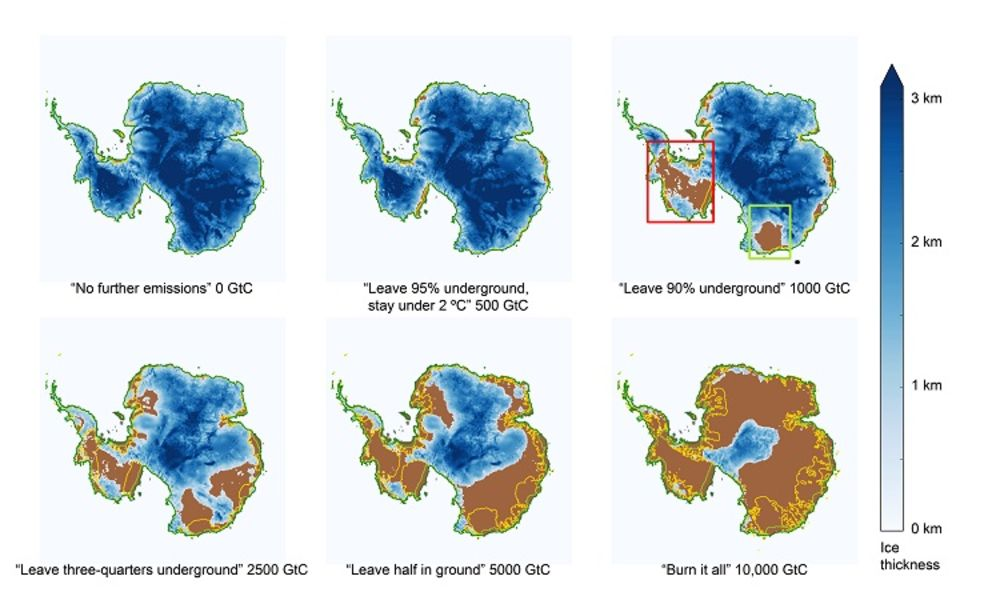
\includegraphics[width=0.8\textwidth]{images/greenlandSeaLevel}
	\caption{Grafik die die Polarschmelzung, nach Ölmenge, illustriert \cite{SIMR.CH2-motorwirkungsgrad.SeaLevelRiseAllOilBurnt}}\label{Fig:imgGreenlandMelting}
\end{figure}

\newpage
\textbf{Zielsetzung\newline}
Gewollt war also ein möglichst kraftstoffeffizienter Schaltvorschlag, doch um verstehen zu können wieso der Schaltvorschlag funktioniert, ist zuerst einiges an Grundwissen nötig.
Jeder der ein Auto fährt kennt diese Formel \textit{Kraftstoffmenge = Strecke * Verbrauch}. So kann man also entweder weniger fahren oder verbrauchsärmer fahren. Wir möchten uns hier auf 2. konzentrieren. Nur konsequent verfolgte Tipps lassen eine echte Veränderung im Verbrauch erkennen, auch das ist einem Großteil der Autofahrer bekannt, doch welche Tipps lohnt es sich anzuwenden? Dazu später mehr, zuerst mehr zu den momentanen Autos und deren physikalische Hintergründe.
Einigen von Ihnen sind Wahrscheinlich die Prozesse hinter einem 4-Takt Motor ein Begriff, trotzdem möchte ich diese hier kurz zusammenfassen und besonders auf die Energieverluste bei diesem Prozess eingehen:

\begin{figure}[!htb]\centering
	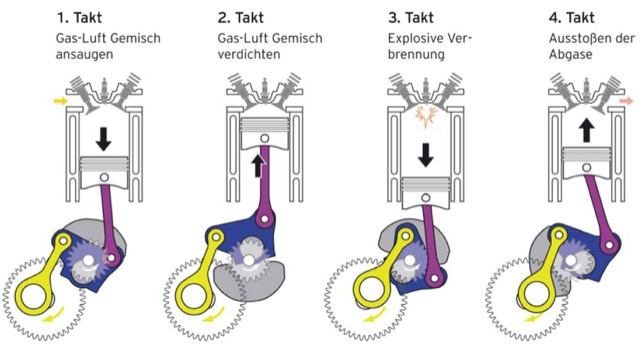
\includegraphics[width=0.8\textwidth]{images/viertaktMotorPrinzip}
	\caption{Prinzip eines 4-Takt Motors \cite{SIMR.CH2-motorwirkungsgrad.4strokeEngine}}\label{Fig:img4strokeEngine}
\end{figure}

Verlorene Energie bei der Verbrennung:
\textit{direktes Zitat: \cite{SIMR.CH1-Fahrstil-Analyse.Motorkennfeld}}
\begin{itemize}
	\item Auspuff: 36\% ausgestoßene Wärme
	\item Durch Zylinderwände: 33\% Abwärme, Teil davon für die Heizung
	\item Motorreibung: Reibung verlangt der Motorbewegung 8\% der Gesamtenergie ab
\end{itemize}
So bleiben im besten Falle 25\% über, die auf die Reifen übertragen werden. Diese 25\% sind zumeist nur unter Volllast erreichbar. Neue TDI Diesel-Motoren schaffen im Optimalfall einen Wirkungsgrad von 30\%, das ist aber bei Verbrennungsmotoren das Optimum. Wenn man nun aber Verbrauchsschonend fährt, so erreicht man meist nur einen Wirkungsgrad von 10\%. \todo{einarbeiten, dass deshalb beim Schaltvorschlag weit gedreht werden muss} Diese wenige Energie die der Motor, aus dem Tropfen Kraftstoff, der eingespritzt wird, erlangt, wird dann durch folgende Widerstände erneut geschwächt:
\textit{direktes Zitat: \cite{SIMR.CH1-Fahrstil-Analyse.Motorkennfeld}}
\begin{itemize}
	\item Beschleunigungswiderstand: Das Beschleunigen eines Körpers braucht Energie. Die Energie wächst quadratisch mit der Geschwindigkeit, sie bleibt aber als \textit{kinetische Energie} in der Geschwindigkeit. 
	\item Steigungswiderstand: Nutzenergie wird beim Bergauffahren gebraucht. Sie bleibt als \textit{potenzielle Energie} gespeichert, welche Abgerufen wird, wenn wieder bergab gefahren wird.
	\item Rollreibung: Diese stellt sich jeder Bewegung in den Weg. Je nach Beschaffenheit der Straße und der Reifen reiben beide aneinander und erwärmen sich. Bei steigender Geschwindigkeit oder niedrigem Reifendruck steigt diese Reibung an.
	\item Luftwiderstand: Diese verdrückt mit zunehmender Geschwindigkeit mehr Energie. Weil bei doppelter Geschwindigkeit nicht nur doppelt so viel Luft verdrängt werden muss, sondern sie auch mit doppelter Geschwindigkeit aufprallt, wächst die bremsende Kraft quadratisch. 
	\item (Bremsen): Dieser Widerstand tritt nicht ständig auf, sondern hängt ausschließlich von seinem Fahrstil ab. Hierbei ist der häufige Wechsel von beschleunigen und bremsen gemeint, was so erneut einen quadratischen Widerstand darstellt. 
\end{itemize}

Alle diese Faktoren sind zumeist von Ihrem eigenen Fahrstil abhängig, welcher dadurch auch Ihren Verbrauch diktiert. Daraus folgt also dass versucht werden muss diese Widerstände durch möglichst effektives Fahren im Straßenverkehr so gering als möglich zu halten.

\textbf{Motorwirkungsgrad\nextline}
Die Zielsetzung des Projektes ist es das Fahrzeug in möglichst hohem Motorwirkungsgrad zu halten, das heißt dass aus jedem Tropfen eingespritztem Kraftstoff möglichst viel Energie gewonnen werden soll. Deshalb wird bei diesem Ansatz auch bewusst dazu aufgefordert den Motor weitaus höher als bei einem konventionellen Schaltvorschlag zu drehen bzw. mit höherer Motorlast zu fahren.
 
Viele Autos bieten im Gegensatz dazu zum Zweck der Verbrauchsmessung nur eine Anzeige des Momentanverbrauchs, welcher wenig hilfreich ist, denn mit dieser Berechnung kann man keine Schlüsse auf die Fahrweise ziehen. Außerdem unterscheiden sich Bordcomputer von einander oft stark. Einige Glätten den Verbrauch auf einen Zeitraum, einige lügen hohe Verbräuche weg, doch alle gemeinsam haben sie, dass die nicht ausreichend dokumentiert sind um faktische Rückschlüsse auf den Fahrstil treffen zu können.

Das ließe sich durch ein einheitliches System aus Hardware und Software vereinheitlichen, wodurch man dann vergleichbare Einheiten, die bei jedem Fahrzeug gleich sind erhalten würde. 

\textbf{Bonanza-Effekt oder Torsionsschwingungen im Antriebsstrang\nextline}
Direktes Zitat: \cite{SIMR.CH2-motorwirkungsgrad.Motorschwingungen}
\textit{
\"Der Verkehr stockt und zwingt den Autofahrer zum Bremsen, er schaltet jedoch nicht in einen niedrigeren Gang. In solchen Fällen ist oftmals ein Brummen zu hören: Die Torsionsschwingung verursacht das unangenehme Geräusch. Sie tritt auf, da sich die Kurbelwelle bei Verbrennungsmotoren nie ganz gleichförmig dreht. Diese Drehschwingung belastet das Getriebe, im schlimmsten Fall leidet die Lebensdauer des Motors – er geht früher kaputt. Auch in anderen Antriebssträngen, die mit einem Verbrennungsmotor gekoppelt sind, kommt es zu dem unerwünschten Effekt – etwa in Schiffen oder Produktionsmaschinen. Grundsätzlich gibt es zwar Lösungen, um ihn ausgleichen. Da die Motoren jedoch immer effizienter werden, nehmen auch die Schwingungen zu – die bestehenden Ausgleichssysteme kommen an ihre Grenzen. Ein Beispiel: Beim PKW geht der Trend zu weniger Zylindern oder aber dazu, einzelne Zylinder zeitweise abzuschalten. Dies hat zur Folge, dass der Motor weniger rund läuft und vermehrt Torsionsschwingungen auftreten. Bei Schiffen entstehen sie, wenn im Hafen von Schweröl oder Dieselantrieb auf Gas umgeschaltet wird, um die Emissionen zu reduzieren.\"}

Demnach ist es also wichtig die Torsionsschwingungen, also Schwingungen in hohem Gang bei niedriger Drehzahl aber hoher Last, zu vermeiden. Diese Schwingungen sind konkret auf dem unten gezeigtem Motorkennfeld im oberen drittel des Drehmoments im Bereich von <1000rpm angesiedelt.

\begin{figure}[!htb]\centering
	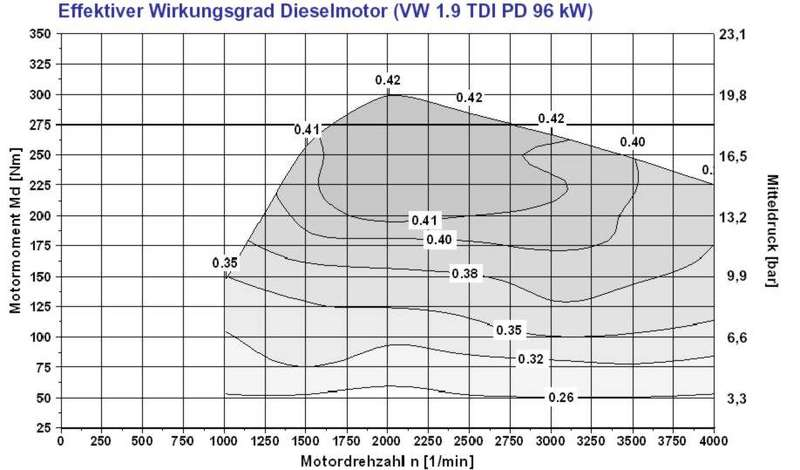
\includegraphics[width=0.8\textwidth]{images/poloMotorkennfeld}
	\caption{Motorkennfeld eines VW Polo, beachten Sie den nicht eingezeichneten Bereich \cite{SIMR.CH2-motorwirkungsgrad.SchwingungenMotorkennfeld}}\label{Fig:imgEngineVibrations}
\end{figure}

%move to the end
Gewollt war also ein möglichst wirkungsgradeffizienter Schaltvorschlag, wobei Herr Prof. Heinz Neuburger, uns diese komplexe Maschinenbau-Thematik sehr verständlich aufbereitete. Durch dieses erlangte Grundwissen war es uns  möglich, auf dieser Information für die konkrete Implementierung aufbauen zu können.
Es wurde zusammenfassend mit Prof. Neuburger festgelegt, dass ein Motor sich nicht mehr innerhalb seines optimalen  Wirkungsgrades befindet, so er 90\% seiner maximalen Drehzahl oder seines Drehmoments erreicht hat, weshalb hochgeschalten werden sollte. Außerdem wurde festgehalten, dass Motorschwingungen äußerst schädlich für Motor und Getriebe sind und deshalb bei auftretenden Schwingungen, bei niedriger Drehzahl und hoher Last, hintergeschalten werden sollte. 

Also kurz:
\begin{itemize}
	\item 90\% der max. Drehzahl oder Drehmoment --> hochschalten, wegen niedrigem Wirkungsgrad
	\item niedrige Drehzahl \&\& hohe Last --> hinunterschalten, wegen Verschleiß durch Motorschwingungen
\end{itemize}

\clearpage % DO NOT REMOVE

\subsection{Hardware und Sensorik}
\lfoot{Autor: Tobias Perny}
\subsubsection{Einleitung}
\label{subsec:Einleitung}

Da das Projekt Bestshift auch die Darstellung von Beschleunigungsdaten, sowie der Innenraumtemperatur umfasst, ist es notwendig eigene Hardware in Form von Sensoren zum KFZ hinzuzufügen.
Hierfür standen mehrere Varianten zur Auswahl:

\begin{itemize}
	\item Smartphone:
	\begin{itemize}
	\item Vorteile: \nextline
	Grundvoraussetzung für den Anwender unseres Systems ist der Besitz eines Smartphones mit einem Android Betriebssystem.
	Das bedeutet, in jedem KFZ unserer Anwender befindet sich ein Smartphone aus welchem Sensorenwerte ausgelesen werden könnten.
	\item Nachteile: \nextline
	Die Sensoren müssen an einer Position im KFZ still stehen und dürfen sich während der Fahrt nicht bewegen. Dies würde bedeuten, dass das Smartphone die gesamte Fahrt über, nicht verwendet werden kann.
\nextline
Desweiteren ist die Auflösung der Sensoren in verschiedenen Smartphones nicht ausreichend für den Anwendungsfall dieses Projektes.
	\end{itemize}
	\item Selbstgebauter Car-PC:
	\begin{itemize}
	\item Vorteile: \nextline
	Einen eigenen PC zu bauen ermöglicht uns die Wahl der passenden Sensoren. Das bedeutet, in jedem Fahrzeug befinden sich der gleiche Car-PC, also dieselben Sensoren.
	Zusätzlich dazu ist es nun bei dieser Variante auch möglich, eine Datenbank auf dem Car-PC zu installieren, und somit Speicher auf dem Smartphone des Benutzers zu sparen.
	\item Nachteile: \nextline
	Ein proprietärer Car-PC muss selbst im Fahrzeug eingebaut werden. Um diesen Nachteil auszugleichen, ist der PC so konzipiert, dass er möglichst einfach in einem DIN-Slot installiert werden kann.
	\end{itemize}
\end{itemize}
\lfoot{Autor: Tobias Perny}
\subsubsection{Vorhandene Umsetzung}
\label{subsec:Vorhandene Umsetzung}
Nach durchgeführte Recherche wurde ein Produkt entdeckt, welches unserem sehr ähnlich ist: der "Low Budget Car PC" von MechLab \cite{MechLab-Enineering}.

\lfoot{Autor: Tobias Perny}
\subsubsection{Single-Board-PC}
\label{subsec:Single-Board-PC}
Ein Single-Board-PC ist ein PC, welcher aus einer einzingen Platine besteht. Auf dieser Platine befinden sich alle Komponenten, die für einen PC als notwendig gelten, mindestens ein Prozessor, RAM. 
\nextline
\textbf{Unterschied zu Mikrocontroller\nextline}
Der wohl größte Unterschied von SBC’s und Microkontrollern ist wohl der, dass Singleboard Computer in der Lage sind ein Betriebsystem auszuführen. Ein Microkontroller wird für weniger komplexe Aufgaben eingesetzt als ein Singleboard Computer.


\clearpage % DO NOT REMOVE
\lfoot{Autor: Tobias Perny}
\subsubsection{Bluetooth}
\label{subsec:Bluetooth}
Bluetooth ist eine kabellose Variante wie mehrere Geräte über kurze Distanz miteinander Kommunizieren können.

\begin{wrapfigure}{r}{0.2\textwidth}
  \begin{center}
    
\includegraphics[width=0.2\textwidth]{images/bluetooth}
  \end{center}
  \caption{Bluetooth Logo, inspiriert vom König von Norwegen und Dänemark, Harald Blauzahn \cite{PERT.CH2-bluetooth.logo}}\label{Fig:imgBluetoothLogo}
\end{wrapfigure}

\textbf{Kommunikation\newline}
Eine Kommunikation mittels Bluetooth kann man in folgende Schritte unterteilen.
\nextline
•	Ein Gerät auswählen mit welchem man kommunizieren möchte
\nextline
•	Herausfinden, wie man mit besagtem Gerät kommunizieren kann
\nextline
•	Aufbauen einer ausgehenden Verbindung
\nextline
•	Akzeptieren einer ankommenden Verbindung
\nextline
•	Senden und empfangen von Daten
\nextline
\textbf{Gerätewahl\nextline}
Jeder Bluetooth Chip besitzt eine eindeutige Adresse. Damit ein Gerät mit einem anderen Kommmunizieren kann, muss es eine Mögllichkeit geben, diese Bluetooth-Adresse zu erfahren. Im Fall von Bluetooth werden dem Gerät meist benutzerfreundliche Namen vom Besitzer oder der Besitzerin vergeben.
Wahl des Transportprotokolles
Die Wahl des Transportprotokolles ist entscheidend für die Art der Datenübertragung. Es gibt mehrere Transportprotokolle, hier werden zwei exemplarisch aufgeführt.
\nextline
\textbf{RFCOMM\nextline}
Bei RFCOMM wird Wert gelegt auf übertragungs Zuverlässigkeit. Es sollen möglichst wenig bis gar keine Pakete verloren gehen. Wenn eine gewisse Menge an Daten nicht in einer bestimmten Zeit gesendet werden kann, wird die Verbindung getrennt und muss neu aufgebaut werden.
\nextline
\textbf{L2CAP\nextline}
Bei diesem Protokoll kommt es nicht auf den Datenverlust an sondern auf die Tatsache das die verbindung stehts aufrecht erhalten wird. Es wird ein Paket so oft gesendet bis es ankommt oder die Verbindung komplett ausfällt.


\clearpage % DO NOT REMOVE
\lfoot{Autor: Tobias Perny}
\subsubsection{I2C}
\label{subsec:I2C}
I2C, Inter Integrated Circuit, ist ein Datenbus bestehend aus zwei Leitungen, einer Datenleitung und einer Taktleitung. Der I2C-Bus eignet sich zur Datenübertragung über kurze Entfernung, beispielsweise auf derselben Platine.

\begin{wrapfigure}{r}{0.2\textwidth}
  \begin{center}
    
\includegraphics[width=0.2\textwidth]{images/i2c}
  \end{center}
  \caption{Logo von i2c \cite{PERT.CH2-i2c.logo}}\label{Fig:imgi2cLogo}
\end{wrapfigure}

\textbf{Grundlagen\newline}
Der I2C-Bus baut auf einem Master-Slave System auf, dass bedeutet es existiert mindestens ein Master und bis zu 127 Slaves auf einem Bus. I2C ist unter anderem ein Multi-Master-Bus, was bedeuted es können mehrere Master zur selben Zeit existieren und der Bus ist noch Lauffähig.
Alle Teilnehmer am Bus erhalten eine eindeutige Adresse. Ein Master kann mithilfe dieser Adresse Daten senden oder empfangen.
\nextline
\textbf{Beispiel\nextline}
Eine Beispielhafte Kommunikation könnte folgendermaßen aussehen:
\nextline
Auf einem I2C-Bus liegt ein Mikrocontroller mit der Adresse 00 und ein Beschleunigungssensor mit der Adresse 01. Der Mikrocontroller übernimmt die Rolle des Masters und der Sensor ist der sogenannte Slave. Nun möchte man Daten aus dem Sensor auslesen. Der Microkontroller prüft ob der Bus „frei“ ist, also ob niemand anderer die Leitung belegt. Dies ist nicht der Fall also sendet der Master eine Nachricht bestehend aus der Zieladresse (in diesem Fall „01“) und teilt dem Slave mit ob Daten gesendet oder empfangen werden sollen. Nun sendet der Slave die Daten an den Controller bis die kommunikation vom Master beendet wird.


\clearpage % DO NOT REMOVE

\subsection{Datenmanagement}
\lfoot{Autor: Daniel Melichar}
Die Speicherung von Daten ist eine der wichtigsten Anforderungen einer jeden Applikation. Ohne gespeicherte Daten können keine Darstellungen, Analysen, oder Verarbeitung geben. Eine Speicherungsmethode muss daher sehr sorgfälltig gewählt werden. Im Folgenden sollen verschiedene Systme betrachtet werden, die für die Datenhaltung im Projekt relevant sind.
\lfoot{Autor: Daniel Melichar}
\subsubsection{Relationale Datenbanken}
\label{subsec:relationaleDB}

Die relationale Datenbank ist seit dem ersten Erscheinen in den 1970er Jahren weit gekommen und ist von den meisten Großkonzernen der Welt adaptiert worden \cite{MELD.CH2-relationaleDB.ranking}. Mit der eigens dafür entwickelten Abfragsprache SQL \textit{(Structured Query Langauge)}war das umgehen mit Datenbanken und Tabellen und der darin gespeicherten Information so einfach wie noch nie.

\begin{figure}[!htb]\centering
	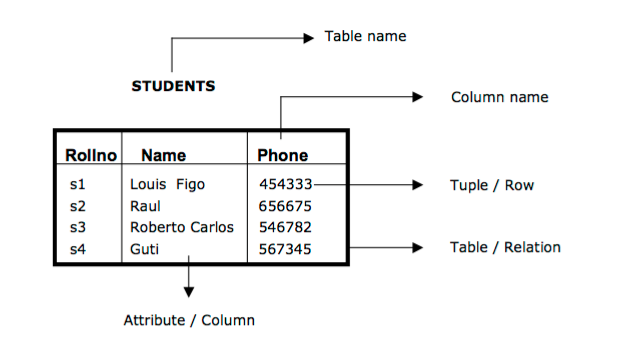
\includegraphics[width=0.8\textwidth]{images/relationaleTabelle}
	\caption{Beispiel einer relationalen Tabelle}
\end{figure}

Features von relationalen DBMS (Achtung: diese sind stark vom eigentlichem DBMS abhängig)
\begin{itemize}
\item Unterstützten eine große Menge an Daten
\item Datensicherheit durch Authentifizierung, Permissions, etc.
\item Fehlertoleranz und Wiederherstellung
\end{itemize}

Hinter den Kulissen sorgt das Relational Database Management System (RDBMS) dafür das die Eigenschaften des ACID Prinzips (Atomicity, Consistency, Isolation, Durability) eingehalten werden. Für eine detailierte Beschreibung zum ACID Prinzip, siehe Sektion \ref{subsec:acidvsbase}. Features der Abrfagsprache SQL, so wie Constraints (primary and foreign keys, Datentype, etc.) oder Stored Procedures/Functions, sorgen dafür, dass ein RDBMS die beste Performance bei simplen Abfragen von mittelgroßen Datemengen hat \cite{MELD.CH2-relationaleDB.performacne}.

Einige der größten Limitierungen \cite{MELD.CH2-relationaleDB.rdbmsBuch} durch das relationale Datenbankmodel sind
\begin{itemize}
\item Skalierbarkeit: Bei komplexen Abfragen in großen Datenbanken sind RDBMS im Vergleich langsamer \cite{MELD.CH2-relationaleDB.performacne}.
\item Komplexität: die Daten müssen zu Tabellen strukturiert werden; es ist also ein Schema notwendig
\item Abfragesprache: Obwohl SQL ein ANSI (American National Standards Institute) Standard ist, gibt es verschiedne versionen der Sprache. Es müssen aber alle hauptfunktionen (wie SELECT, UPDATE, DELETE, INSERT, WHERE) gegeben sein um den ANSI Standard zu erfüllen.
\end{itemize}

Die Verwendung eines relationalen Datenbankmanagementsystem macht also dann Sinn, wenn ein Datenschema erstellt werden kann, also wenn bekannt ist, welche konkreten Daten gesammelt werden und wie diese in Tabellen mit Beziehungen verarbeitet werden können. Durch die SQL Abfragesprache bekommt der Datenbank-Administrator alle Features die er braucht um das System in takt zu halten.
\lfoot{Autor: Daniel Melichar}
\subsubsection{Nicht relationale Datenbanken (NoSQL)}
\label{subsec:nichtrelationaleDB}

In diesem Kapitel werden ein Einblick in das Konzept von nicht-relationalen Datenbanken gegeben. Es wird nicht über die ersten Systeme gesprochen die damals dem NoSQL-Movement angehörten (Objekt-Datenbanken, XML-Datenbanken, Datenbanken für spezielle Anwendungsgebiete wie Analyse oder Streamprozessoren) diese sollten aber zumindest erwähnt werden.

\textbf{Motive und Beweggründe\newline}
Der Term \textit{NoSQL} wurde erstmalig in 1998 für eine relationale Datenbank, welche ohne der SQL-Sprache funktioniert, verwendet\cite{MELD.CH2-noSQL.firstSQLNaming}. Der Term wurde dann wieder in über die Jahre von verschiedensten Leuten aufgenommen. Unglücklicherweise gab es keine definitive Beschränkung für welche Datenbanksysteme zum NoSQL-Movement gehören. Durch den Blogger und Rackspace Mitarbeiter, Eric Evans, ist der Term ganz besonders bekannt geworden – er sagte hierzu: \cite[\textit{“the whole point of seeking alternatives is that you need to solve a problem that relational databases are a bad fit for”}]{MELD.CH2-noSQL.whatsInAName}. NoSQL Datenbanken wurden hauptsächlich von Großkonzernen für den Eigenbedarf entwickelt (Amazon’s Dynamo, Google’s BigTable, LinkedIn’s Voldemort, Facebook’s Cassandra, Yahoo!’s PNUTS). Diese Großkonzerne haben den relationalen Ansatz nicht komplett verworfen, sie fanden lediglich, dass das Model nicht den Anforderungen entspricht\cite{MELD.CH2-noSQL.capTheoremComp}.

Das bekannte IT und Technologie Magazine \textit{Computerworld} hat in 2009 bei einer NoSQL Konferenz in San Franciso die dort vorhanden Developer befragt wieso NoSQL gegenüber relationalen Datenbanken im Vorteil liegt\cite{MELD.CH2-noSQL.whyItsBetter}.

Die folgenden Erklärungen wurden von den Entwicklern gemacht.
\begin{itemize}
	\item \textbf{Unnötige Komplexität wird vermieden}\newline
	 Relationale Datenbanken verfügen über eine große Anzahl an Features und strikter Daten Konsistenz Vorschriften. Jedoch kann diese Anzahl an Features und die Anbindung an das ACID-Model zu viel für spezifische Anwendungsfälle sein. Zum Beispiel ist die Überprüfung von Session Daten die Mehrmals als Kopie abgespeichert sind nicht notwendig.

	\item \textbf{Hohe Verarbeitungsmenge}\newline
	 Manche NoSQL Datenbanken verfügen über eine weitaus größere 	Verarbeitungsmenge. So wird bei dem column-store Hypertable, welches die Ziele von Google’s BigTable verfolgt, erlaubt es bis zu einer Millionen Datensätze pro Tag zu speichern. Ein weiteres Beispiel ist Google’s BigTable selbst; es kann bis zu 20 Petabyte pro Tag verarbeiten.

	\item \textbf{Horizontale Skalierbarkeit und geringe Hardware requirements}\newline
	 Im Vergleich mit relationalen DBMS sind die meisten NoSQL Datenbanken so konzipiert um horizontale Skalierung möglichst einfach durchzuführen. Horizontale Skalierung bedeutet prinzipiell mehr Server, oder im allgemeinen Verarbeitungsmachinen, in den Pool der Ressourcen hinzu zu fügen. Es gibt zwar auch eine äquivalente Verbesserungsmöglichkeitne für RDBMS, das so genannte \textit{sharding}, dies ist oft aber weit aus komplizierter als bei NoSQL. Zum Beispiel gibt es bei der Bekannten NoSQL Datenbank \textit{MongoDB} eine automatische Version der Sklaierung.

	\item \textbf{Object-Relational Mapping wird vermieden}\newline
	 Auch hier verwenden die meisten NoSQL Datenbanken eine Struktur zur Speicherung der Daten die entweder sehr Simple oder sehr Ähnlich zu jenen sind die auch bei Objekt-Orientierten-Programmiersprachen aufzufinden sind. Hierfür ist dann kein ressourcenintensives Object-Relational Mapping notwendig.
\end{itemize}

Zu diesem Bericht gab es dann auch einen Blog post von Nati Shalom, CTO und Gründer von GigaSpaces. Er hat die folgenden weiteren Punkte für die NoSQL-Bewegung aufgestellt\cite{MELD.CH2-noSQL.natiShalomlol}.

\begin{itemize}
	\item \textbf{Komplexität und benötigter Aufwand bei Datenbank Clustern}\newline
	 Er meint, dass NoSQL Datenbanken auf eine Art und Weise entwickelt worden sind, die das erstellen von Clustern sehr einfach macht. Unter anderem spielt hier auch das bereits angesprochene Skalieren auf horizontaler Ebene eine große Rolle.
	
	\item \textbf{Kompromiss zwischen Performance und Verlässlichkeit}\newline
	 Shalom behauptet außerdem, dass verschiedene Szenarien gibt, in welchen Applikationen den Fokus auf Performance legen und nicht auf Verlässlichkeit. Ein gutes Beispiel für dieses Szenario sind die Daten von HTTP Sessions – diese müssen zwischen vielen Web Servern geschickt werden, löschen sich aber dann sobald der User sich abmeldet.

	\item \textbf{Cloud Computing}\newline
	 Hier werden sehr oft NoSQL Lösungen verwendet, da dass Limit der Skalierbarkeit sehr hoch, bis sogar unendlich ist, es wenig administrative Tätigkeiten im Umgang mit NoSQL gibt, es viele NoSQL Datenbanken gibt die spezifisch für Datawarehousing entiwckelt worden sind, uvm.
\end{itemize}

\textbf{Techniken und Konzepte\newline}
\htab\textbf{Das CAP-Theorem\newline}
Das von Eric Brewer im Jahre 2000 entwickelte CAP-Theorem ist heutzutage in vielen Web-Unternehmen (z.B. Amazon) aber auch in der NoSQL Community aufzufinden\cite{MELD.CH2-noSQL.capTheorem}. Der CAP Akronym steht für:

\begin{itemize}
	\item \textit{Consistency:} Ob und wie ein System in den konsistenten Zustand, nach Ausführung einer Operation, zurück gelangt. Ein verteiltes System wird im Normalfall als Konsistent bezeichnet, wenn alle lesenden Teile das selbe Resultat aus dem geteilten Informationspool bekommen.

	\item \textit{Availability:} Hierbei ist vor allem auf das Design und Umsetzung eines Systems zu achten. Es sollte so entwickelt sein, dass bei Ausfall eines Servers in einem Cluster immer noch die selben Operationen durchgeführt werden können.

	\item \textit{Partition Tolerance:} Anders als bei Availability geht es hier meistens um Netzwerk Partitionen und die Möglichkeit weiter Operationen durchzuführen, wenn zwei Netzwerke im System nicht miteinander kommunizieren können.
\end{itemize}

 Brewer behauptet, dass man nur zwei von diesen drei Eigenschaften in einem \textit{shared-data system} haben kann\cite{MELD.CH2-noSQL.capTheorem}. In seiner Präsentation hat er über die Vor- und Nachteile von ACID und BASE Systemen (siehe nächsten Paragraphen) geredet und einige Entscheidungskriterien vorgestellt um sich für eine der beiden Modelle zu entscheiden: wenn ein System, oder Teile eines Systems, konsistent und Partition-Tolerant sein müssen, sind ACID Eigenschaften benötigt; wenn Verfügbarkeit und Partition-Tolerants benötigt werden, sollte das System mittels BASE Eigenschaften erstellt werden. Anhand folgender Tabelle, welche direkt aus seiner Präsentation genommen wurde, lässt es sich am besten veranschaulichen.

\begin{table}[!htb]
\centering
\begin{tabular}{|l|l|l|}
\hline
\multicolumn{1}{|c|}{\textbf{Choice}} & \multicolumn{1}{c|}{\textbf{Traits}} & \multicolumn{1}{c|}{\textbf{Examples}} \\ \hline
Consistence + Availability & \begin{tabular}[c]{@{}l@{}}2-phase-commit\\ cache-validation protocols\end{tabular} & \begin{tabular}[c]{@{}l@{}}Single-site databases\\ Cluster databases\\ LDAP\\ xFS file system\end{tabular} \\ \hline
Consistency + Partition tolerance & \begin{tabular}[c]{@{}l@{}}Pessimistic locking\\ Make minority partions unavailable\end{tabular} & \begin{tabular}[c]{@{}l@{}}Distributed databases\\ Distributed locking\\ Majority protocols\end{tabular} \\ \hline
Availability   + Partition tolerance & \begin{tabular}[c]{@{}l@{}}expirations/leases\\ Conflict resolution\\ Optimistic\end{tabular} & \begin{tabular}[c]{@{}l@{}}Coda\\ Web caching\\ DNS\end{tabular} \\ \hline
\end{tabular}
\caption{CAP-Theorem – Alternatives, Traits, Examples \cite{MELD.CH2-noSQL.capTheorem}}
\end{table}

Grundsätzlich kann man sagen, dass bei relationalen Datenbanken weniger Availability herscht als bei der NoSQL Variante. Beide Systeme verfügen jedoch über Partition Tolerance\cite{MELD.CH2-noSQL.capTheoremComp}

\begin{figure}[!htb]\centering
	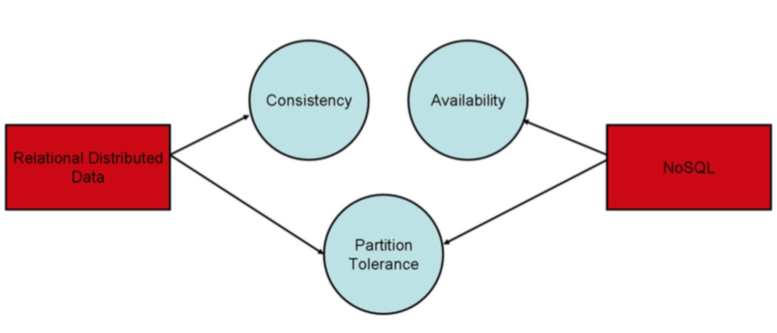
\includegraphics[width=0.8\textwidth]{images/capTheorem}
	\caption{CAP-Theorem bei RDBMS und NoSQL\cite{MELD.CH2-noSQL.capTheoremComp}}
\end{figure}

\textbf{ACID vs BASE\newline}
Das Internet erzeugt Tag für Tag für eine enorme Menge an Daten welche verarbeitet, analysiert und bereitgestellt werden müssen. Die Applikationen und Service in diesem Bereich müssen den individuellen Bedarf an Performance, Zuverlässigkeit, Betriebsbereitschaft, und Konsistenz feststellen. Wie bereits beim CAP-Theorem beschrieben können diese Applikationen und Service nur zwei Optionen von Consistency, Availability, und Partition Tolerance, genommen werden. Immer mehr Applikationen und Service bevorzugen die Option von Availability und Partition Tolerance und vernachlässigen somit die strikte Toleranz. Diese Eigenschaften sind schwer mit dem ACID Model zu erreich, jedoch wurde dafür das BASE Model entwickelt. Es gibt kein Model das besser ist, man muss das richtige Model für seine Bedürfnisse wählen.

Das Akronym BASE steht für folgende Eigenschaften
\begin{itemize}
	\item Basically Available
	\item Soft-state
	\item Eventual consistency
\end{itemize}

Brewer stellt den Vergleich zwischen ACID und BASE mit der Darstellung, welche man in der Tabelle sehen kann. Es ist jedoch zu beachten das diese beiden Konzepte sich nicht aufheben sollen, sondern ein großes Spektrum an Möglichkeiten bieten sollen. 

\begin{table}[!htb]
\centering
\label{acidvsbaseTable}
\begin{tabular}{|l|l|}
\hline
\multicolumn{1}{|c|}{\textbf{ACID}} & \multicolumn{1}{c|}{\textbf{BASE}} \\ \hline
\begin{tabular}[c]{@{}l@{}}Strong consistency \\ Isolation \\ Focus on “commit” \\ Nested transactions \\ Availability? \\ Conservative (pessimistic) \\ Difficult evolution (e.g. schema)\end{tabular} & \begin{tabular}[c]{@{}l@{}}Weak consistency – stale data OK \\ Availability first\\ Best effort \\ Approximate answers OK \\ Aggressive (optimistic)\\ Simpler!\\ Faster \\ Easier evolution\end{tabular} \\ \hline
\end{tabular}
\caption{ACID vs BASE \cite{MELD.CH2-noSQL.capTheorem}}
\end{table}

\textbf{Partitionierung\newline}
Ab einer gewissen Menge an Daten werden die benötigten Ressourcen über die Kapazität einer einzelnen Maschine hinaus laufen. In diesem Fall müssen die Daten über mehrere Maschinen aufgeteilt werden – das nennt man \textit{Partitioning}. Hierbei gilt es auch zu beachten, dass  das System weiterhin funktionsfähig sein muss, wenn einer dieser Maschinen ausfällt. Es sollte auch beachtet werden, dass die Last der Ressourcen auf alle Server aufgeteilt ist (\textit{load balancing}).

Bei NoSQL Datenbanken gibt es hierfür verschiedene Konzepte um die Best möglichen Ergebnisse zu erhalten.

\begin{description}
	\item[Memory Caches] können als separate Zwischenspeicher (z.B. RAM) Datenbanken geshene werden. Hierbei werden die am meist gebrauchten Daten mit einer hohen Frequenz in den Memory gespeichert und somit eine Art von Caching entwickelt. In den meisten Fällen hollt man sich dann die Daten über eine API und einen speziellen Key.

	\item[Clustering] von Datenbanken ist eine weitere Möglichkeit. Hierbei ist es vor allem sehr wichtig, dass der Verwendet der Applikaion gar nicht mit bekommt mit wie vielen Servern er kommuniziert.

	\item[Trennung von Read und Write] bedeutet, dass es spezifische Server gibt die nur Schreiben, bzw. nur Lesen dürfen. Durch die asynchrone Verarbeitung der Daten gibt es beinahe keinen lag zwischen den Servern und durch Replikation der Daten (Mehrfachspeicherung) ist es auch schwierig die Daten zu verlieren

	\item[Sharding] ist ein Prinzip in welchem die Daten so gespeichert sind, dass die Antworten auf die Requests nahe zusammenliegen selbst auf einem einzigen Server. Auch hier spielt bei mehreren Servern die Verteilung eine große Rolle. Die konkrete Umsetzung von Sharding ist eine mathematisch sehr komplizierte und würde den Rahmen sprengen.
\end{description}

\textbf{Kritik\newline}
Selbstverständlich gibt es nicht nur positive Dinge über NoSQL. Auch nicht relationale Systeme haben einige Punkte in welchen es noch Verbesserungsbedarf gibt \cite{MELD.CH2-noSQL.sqlvsnosql}. 

\begin{itemize}
	\item \textbf{Vortschritt\\}
	Relationale Datenbanken existierten schon um einige Jahre länger als die NoSQL Variante. Die Zielsetzung von RDBMS ist es stabil und verlässlich zu sein - was teilweise auch bedeutet, dass es wenige neue Innovationen gibt. Hingegen gibt es noch einige NoSQL Datenbanksysteme die ein Basis Feature-Set entwickeln müssen.

	\item \textbf{Support\\}
	Auch hier spielt die etwas längere Lebensdauer von RDBMS eine große Rolle. Solche Namen wie \textit{MySQL, PostgreSQL, Microsoft SQL Server} sind sehr bekannt in der IT Welt. Die Entwickler dieser Systeme setzen auch auf einen guten Support, wobei dieser oft nur for Enterprise Editions zur Verfügung steht. Hingegen sind die meisten NoSQL Datenbanken Open Source, und haben daher meist nur Community Support. Ob dieser Ansatz gut oder schlecht ist eine Ansichtssache von Open Source Projekten.

	\item \textbf{Administration\\}
	Der wahrscheinlich größte negative Aspekt von NoSQL ist die eigentliche Administration. Es wird zwar oft gesagt, dass NoSQL keine administrativen Tätigkeiten benötigt, in den meisten Fällen muss aber trotzdem hin und wieder an der Datenbank gefeilt werden. Bei relationalen Datenbanken gibt es durch Einsatz von Persmissions, Rollen, und durch das ACID-Model weit aus einfache administrative Möglichkeiten.

	\item \textbf{Fehlende Standardisierung\\}
	Bei relationalen Datenbanken gibt es zwar auch eine einheitliche Programmiersprache die prinzipiell für alle DBMS funktioniert, aber auch hier gibt es verschiedene Dialekte. Bei NoSQL Datenbanken ist es dem Entwickler überlassen wie er mit der Datenbank kommunizieren will. In den meisten Fällen wird JavScript verwendet, es kann aber auch eine eigene, komplett neue Programmier- oder Skriptsprache sein.
\end{itemize}

\textbf{Klassifikation von NoSQL Datenbanken\newline}
Zum Zeitpunkt der Erstellung dieses Dokuments gibt es weit über zweihundert NoSQL Datenbanken\cite{MELD.CH2-noSQL.listOfNoSQLDB}. All diese Datenbanken können in vier Kategorien eingeteilt werden:

\begin{itemize}
	\item Key-Value Stores
	\item Column-Oriented Databases
	\item Document Databases
	\item Graph Stores
\end{itemize}

Für eine detailierte Beschreibung, Anwendungsfälle, und Vergleiche, siehe Sektion \ref{subsec:dbms}

\clearpage
\lfoot{Autor: Daniel Melichar}
\subsubsection{Datenbankmanagementsysteme}
\label{subsec:dbms}

In der folgenden Sektion werden die gängisten RDBMS und NoSQL Datenbanken vorgestellt und gegeneinander Vergleicht. Es ist zu beachten, dass es ein wenig mehr zu NoSQL Datenbanken gibt, da wir mit einer solchen arbeiten (siehe \ref{subsec:datenmanagementimpl}).

\paragraph{Relationale DBMS\nextline}
\tab\textbf{MySQL\newline}
Dieses RDBMS wurde ursprünglich entwickelt als \textit{lightweight database-like engine} und hatte in den ersten Versionen wenige von den Features die zu dem Zeitpunkt als essentiell gekennzeichnet waren. Trotz allem war es ein nützliches Tool, welches zwar kein eigentliches RDBMS war, aber dennoch einfach zum Einrichten und Verwenden war.

In den letzten Jahren ist MySQL von dem ursprünglichen Weg abgekommen – es hat sich zu einem kompletten RDBMS entwickelt.  Trotz Bekanntheit wird MySQL immer noch nicht als die stabilste Datenbank, oder jene mit dem größten Feature-Set, angesehen.

Alles im allen wird MySQL (oder Klone) in den meisten Fällen verwendet.

\tab\textbf{Oracle\newline}
Dieses DBMS ist bekannt für seine große Anzahl an Features und dem größten Marktanteil. Vergleicht man Oracle mit anderen Datenbanken wird schnell klar, dass andere Datenbanken bei weitem nicht so viel können wie Oracle. Beinahe jedes Betriebssystem wird unterstützt; fast jede Programmiersprache hat Einbindungen die es ermöglichen mit einer Oracle Datenbank zu sprechen; Serverseite Programmierung hat viele Möglichkeiten; die Performance von Oracle Datenbanken ist exzellent; uvm.

Es gibt aber zwei große, negative Aspekte welche Oracle für viele nicht verwendbar machen: kosten und die Komplexität von Administration

\tab\textbf{PostgreSQL\newline}
\todo{Content}

\tab\textbf{SQL Server\newline}
\todo{Content}

\begin{table}[!htb]
\centering
\label{rdbms-comp}
\resizebox{\columnwidth}{!}{%
\begin{tabular}{|l|l|l|l|l|}
\hline
\textbf{Name} & \multicolumn{1}{c|}{\textbf{Microsoft SQL Server}} & \textbf{MySQL} & \textbf{Oracle} & \textbf{PostgreSQL} \\ \hline
\textbf{Website} & www.microsoft.com/sqlserver & www.mysql.com & www.oracle.com/database & www.postgresql.org \\ \hline
\textbf{Developer} & Microsoft & Oracle & Oracle & \begin{tabular}[c]{@{}l@{}}PostgreSQL Global\\ Development Group\end{tabular} \\ \hline
\textbf{\begin{tabular}[c]{@{}l@{}}Erster \\ Release\end{tabular}} & 1989 & 1995 & 1980 & 1989 \\ \hline
\textbf{\begin{tabular}[c]{@{}l@{}}Momentaner \\ Release\end{tabular}} & \begin{tabular}[c]{@{}l@{}}SQL Server 2014\\ April 2014\end{tabular} & \begin{tabular}[c]{@{}l@{}}5.7.11\\ February 2016\end{tabular} & \begin{tabular}[c]{@{}l@{}}12 Release 1 (12.1.0.2)\\ July 2014\end{tabular} & \begin{tabular}[c]{@{}l@{}}9.5.1\\ February 2016\end{tabular} \\ \hline
\textbf{Lizens} & Kommerziell & Open Source / Kommerziell & Kommerziell & Open Source \\ \hline
\textbf{\begin{tabular}[c]{@{}l@{}}Entwickelt\\ in..\end{tabular}} & C++ & C und C++ & C und C++ & C \\ \hline
\textbf{\begin{tabular}[c]{@{}l@{}}Unterstütze\\ Server\\ Systeme\end{tabular}} & Windows & \begin{tabular}[c]{@{}l@{}}FreeBSD\\ Linux\\ OS X\\ Solaris\\ Windows\end{tabular} & \begin{tabular}[c]{@{}l@{}}AIX\\ HP-UX\\ Linux\\ OS X\\ Solaris\\ Windows\\ z/OS\end{tabular} & \begin{tabular}[c]{@{}l@{}}FreeBSD\\ HP-UX\\ Linux\\ NetBSD\\ OpenBSD\\ OS X\\ Solaris\\ Unix\\ Windows\end{tabular} \\ \hline
\textbf{\begin{tabular}[c]{@{}l@{}}Unterstütze\\ Sprachen\end{tabular}} & \begin{tabular}[c]{@{}l@{}}.NET\\ Java\\ PHP\\ Python\\ Ruby\\ Visual Basic\end{tabular} & \begin{tabular}[c]{@{}l@{}}Ada\\ C\\ C\#\\ C++\\ D\\ Eiffel\\ Erlang\\ Haskell\\ Java\\ Objective-C\\ OCaml\\ Perl\\ PHP\\ Python\\ Ruby\\ Scheme\\ Tcl\end{tabular} & \begin{tabular}[c]{@{}l@{}}C\\ C\#\\ C++\\ Clojure\\ Cobol\\ Eiffel\\ Erlang\\ Fortan\\ Groovy\\ Haskell\\ Java\\ JavaScript\\ Lisp\\ Objective-C\\ OCaml\\ Perl\\ PHP\\ Python\\ R\\ Ruby\\ Scala\\ Tc\\ Visual Basic\end{tabular} & \begin{tabular}[c]{@{}l@{}}.NET\\ C\\ C++\\ Java\\ Perl\\ Python\\ Tcl\end{tabular} \\ \hline
\textbf{\begin{tabular}[c]{@{}l@{}}APIs und \\ andere Verbindungs-\\ möglichkeiten\end{tabular}} & \begin{tabular}[c]{@{}l@{}}OLE DB\\ Tabular Data Stream (TDS)\\ ADO.NET\\ JDBC\\ ODBC\end{tabular} & \begin{tabular}[c]{@{}l@{}}ADO.NET\\ JDBC\\ ODBC\end{tabular} & \begin{tabular}[c]{@{}l@{}}ODP.NET\\ Oracle Call Interface (OCI)\\ JDBC\\ ODBC\end{tabular} & \begin{tabular}[c]{@{}l@{}}Native C Libary\\ ADO.NET\\ JDBC\\ ODBC\end{tabular} \\ \hline
\end{tabular}
}
\caption{Vergleich von relationalen Datenbankmanagementsystemen \cite{MELD.CH2-dbms.compRDBMS}}
\end{table}

\clearpage

\paragraph{NoSQL Datenbanken\newline}

Im allgemeinen gibt es vier Arten von NoSQL Datenbanken\cite{MELD.CH2-dbms.compNoSQLInfo}: Key-Value Stores, Column-Oriented Databases, Document Databases und Graph Stores. Selbstverständlich gibt es auch eigens entwickelte Datenbanken die nicht in diese vier Kategorien eingeteilt werden können, diese vier sind aber jene die am meisten verwendet werden.

\begin{itemize}
	\item \textbf{Key-Value Stores\newline}
	Diese Art von Datenbank ist prinzipiell ziemlich simple, aber dennoch effizient und schnell. In den meisten Fällen kommuniziert man mit der Datenbank mittels einer API die für mehrere Programmiersprachen zur Verfügung gestellt wurde. In den meisten Fällen wird der Key mittels Strings realisiert und dieser referenziert auf die Values (also die eigentlichen Daten). Diese Datenbanken sind Hash-Tabellen sehr ähnlich, da auch hier der Key als Index verwendet wird und somit schnelle Zugriffszeiten ermöglicht werden. Wie bei den meisten NoSQL Datenbanken ist auch bei Key-Value kein Schema aufzufinden.

	Beispielhafte Anwendungen von Key-Value Datenbaken wären die Speicherung von Session Daten eines Users, die Speicherung der Artikel in einem Einkaufswagen, oder die Speicherung der beliebten Produkte.

	Bekannte Key-Value Datenbanken: Amazon DynamoDB und RIAK

	\begin{figure}[!htb]\centering
		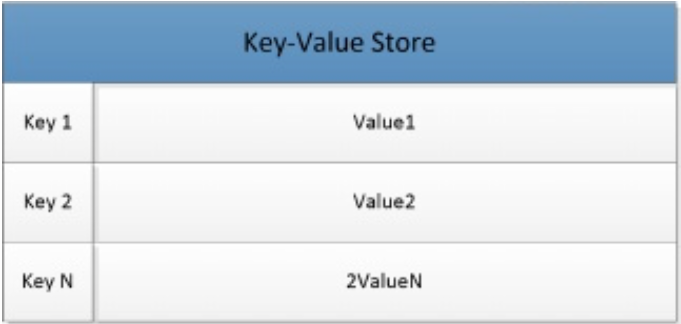
\includegraphics[width=0.5\textwidth]{images/keyvalueStore}
		\caption{Aufbau von Key-Value Datenbanken}
	\end{figure}

	\clearpage

	\item \textbf{Column-Oriented Databases\newline}
	Column Stores in NoSQL sind eigentlich eine Mischung aus Row/Column Stores anders als bei relationalen column Datenbanken. Es herrscht zwar das selbe Konzept von Zeile-nach-Zeile wie bei relationalen Datenbanken, aber diese werden nicht in Tabellen gespeichert, sondern in massiven, verteilten Architekturen. Jeder Key ist mit einer oder mehreren Attributen verknüpft. Diese Art von Datenbank ist grundsätzlich so aufgebaut das mit einem einzigen Befehl eine große Menge an Daten zurückgebracht werden kann. 

	Column Store Datenbanken werden sehr oft für Data Mining, Datawarehousing und im Allgemeinen für Business Analytics verwendet.

	Einige der Bekanntesten Datenbanken sind: Googe BigTable, Cassandra

	\begin{figure}[!htb]\centering
		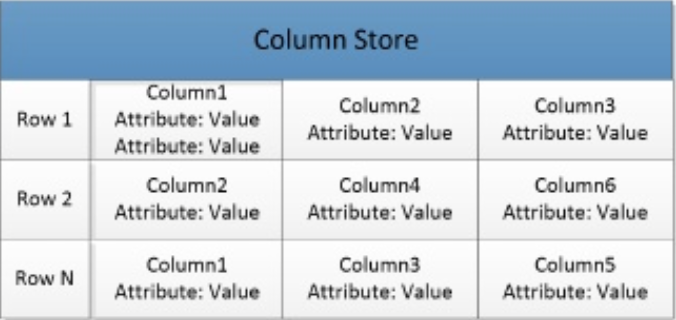
\includegraphics[width=0.5\textwidth]{images/columnStore}
		\caption{Aufbau von Column-Oriented Datenbanken}
	\end{figure}

	\clearpage

	\item \textbf{Document Databases\newline}
	Document Store Database sind jene Datenbanken die Daten in Form von Files ablegen und speichern. Hierbei ist vor allem auf die Performance und horizontale Skalierbarkeit zu achten. Die Files, oder Dokumente, in einer Document-Oriented Datenbank sind ähnlich zu jenen einer relationalen Datenbank, aber der große Unterschied hierbei ist, dass diese an kein Schema gebunden sind und somit um einiges flexibler sind. Es werden oftmals standardisierte Formate wie XML, PDF oder JSON verwendet. Diese Dokumente sind mittels einem eindeutigen Key adressiert welcher das File auch repräsentiert. Diese Keys können einfache Strings oder ganze Pfade sein.

	Anwendungsgebiete von dieser Art von Datenbank sind Applikationen wie Content Management Systeme, Blog Software, usw. 

	Die bekanntesten Document-oriented Datenbanken sind: MongoDB und CouchDB

	\begin{figure}[!htb]\centering
		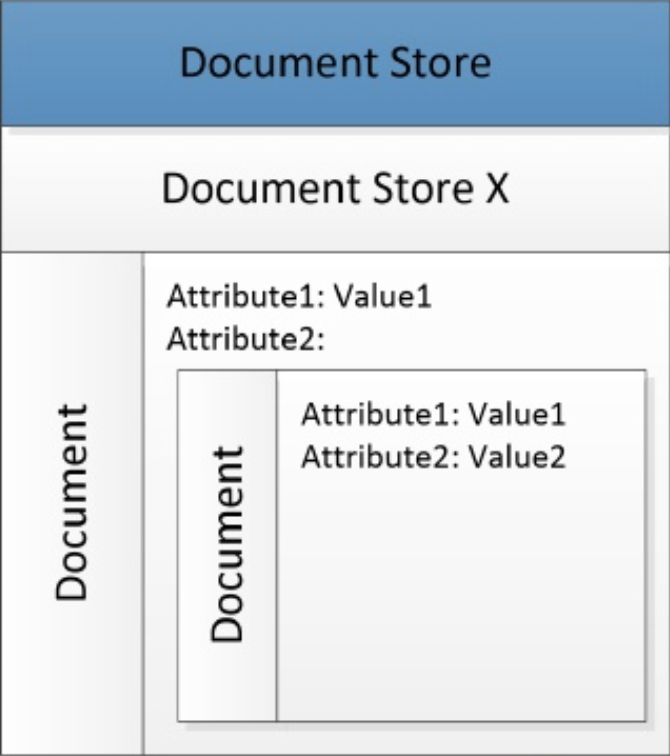
\includegraphics[width=0.5\textwidth]{images/documentStore}
		\caption{Aufbau von Document Datenbanken}
	\end{figure}

	\clearpage

	\item \textbf{Graph Stores\newline}
	In Graph Datenbanken werden die Daten mittels so genannten Nodes und Edges gespeichert, wobei Nodes als Objekte arbeiten und Edges und die Beziehungen zwischen den einzelnen Objekten. Es wird hier die \textit{Index-Free-Adjacency} Technik verwendet. Das bedeutet, dass jeder Node mit Pointern versetzt wurde die es ermöglichen auf den nächstgelegenen Node zugriff zu bekommen. Somit kann mit einem Befehl über mehrere Nodes iteriert werden. In Graph-Oriented Datenbanken liegt der Hauptsächliche Fokus auf die Verbindung zwischen den Daten, also in welcher Beziehung diese stehen. Anders als bei anderen NoSQL Datenbanken wird bei Graph Datenbanken oftmals teile des ACID Models verwendet.

	Sozialle Netzwerke sind die hauptsächlichen Anwendungsgebiete von Graph Datenbanken, aber auch Applikationen für Sicherheits- und Zugriffskontrollen, Content Management Systeme, Cloud Management, etc. 

	Die am verbreitete Graph Datenbank ist ohne Zweifel Neo4j

	\begin{figure}[!htb]\centering
		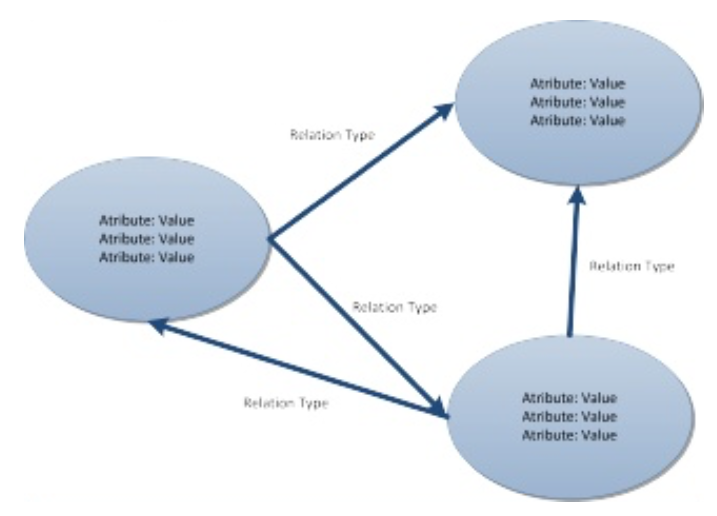
\includegraphics[width=0.5\textwidth]{images/graphStore}
		\caption{Aufbau von Document Datenbanken}
	\end{figure}
\end{itemize}
\clearpage

Hier kann man nochmalsd jene NoSQL Datenbanken betrachten und vergleichen die zum hautigen Zeitpunkt am meisten verwendet werden.

\begin{figure}[!htb]\centering
	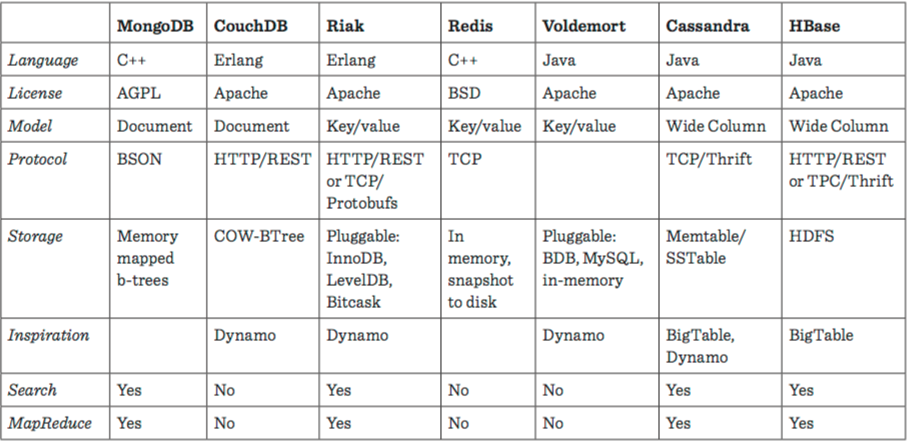
\includegraphics[width=1\textwidth]{images/noSQLComp}
	\caption{Vergleich von gängigen NoSQL Datenbanken\cite{MELD.CH2-dbms.compNoSQL}}
\end{figure}


\clearpage % DO NOT REMOVE

\subsection{Android Development}

\lfoot{Autor: Fitim Faiku}
\subsubsection{Grundsätze einer Android Applikation}
\label{subsec:aapp-fundam}

Android Apps werden in der Programmiersprache Java geschrieben.
Die Android SDK-Tools kompilieren Code zusammen mit allen Ressourcen-Dateien in eine APK.
Eine APK ist ein Android-Paket, welches alle Inhalte einer Android App enthält. 
Die APK-Datei wird dann auf das Android-Gerät installiert. 


\textbf{Native vs HTML5 vs Hybrid}
\todo{Überschrift anders?}
Bei der Umsetzung unserer Android Applikation, hatten wir die Entscheidung, wie wir die Android App erstellen. 
Da Android mehrere Programmierarten unterstützt musste evaluiert werden welche Programmiermodule für unsere App am Besten geeignet ist. \nextline

\textbf{Native\newline} 
Für native Apps wird auf der Android-Plattform die Sprache Java verwendet.
Native Apps zeigen die beste Performance.
Die Dokumentation zu Native Apps ist am Besten, da es über 2500 Bücher zur Android Entwicklung gibt.
Für Nativ Apps werden Entwicklungsumgebungen-IDE(Integrated Developement Enviroment) verwendet um die gewünschte App zu Programmieren.\nextline

\textbf{HTML5\newline} 
HTML5 verwendet die Standard Web Technologien, wie JavaScript und CSS.
HTML5 Applikationen werden über Browser abgespielt, wobei jedes Gerät auf die Browser zugreifen kann und dadurch die App auf mehreren Plattformen abgespielt werden kann. \nextline

\textbf{Hybrid\newline} 
Hybrid Apps sind eine Mischung aus nativ und HTML5 Apps. Hybrid bietet das Beste aus beiden Welten. Das Design wird mittels HTML5 und CSS erstellt, wobei sich dahinter ein JavaScript-Code befindet. Hybrid Apps sind genauso auf jede Plattform abspielbar, wobei sie für die Plattform entsprechend umprogrammiert müssten.    
\nextline

\clearpage % DO NOT REMOVE
\lfoot{Autor: Fitim Faiku}
\subsubsection{Kompatible Geräte}
\label{subsec:device-compability}

Android kann auf vielen verschiedenen Plattformen, wie Handys oder Tabletts laufen.
Als Entwickler bietet die Palette von Geräten ein enormes potenzielles Publikum.
Um auf all diesen Oberflächen reibungslos zu funktionieren muss eine App einige Feature Variabilitäten tolerieren und eine 
flexible Benutzeroberfläche zur Verfügung stellen. 

Um das zu ermöglichen bietet Android die Möglichkeit, verschiedene XML Layouts zu erstellen um verschiedene Bildschirmgrößen anzusprechen.

Beim Programmieren der App kann auch die minimale und maximale kompatible Android-Version des Devices eingestellt werden, wobei hier eine möglichst umfangreiche Auswahl der Versionen einen größeren Umfang an Nutzern erzielt.

\begin{figure}[!htb]\centering
	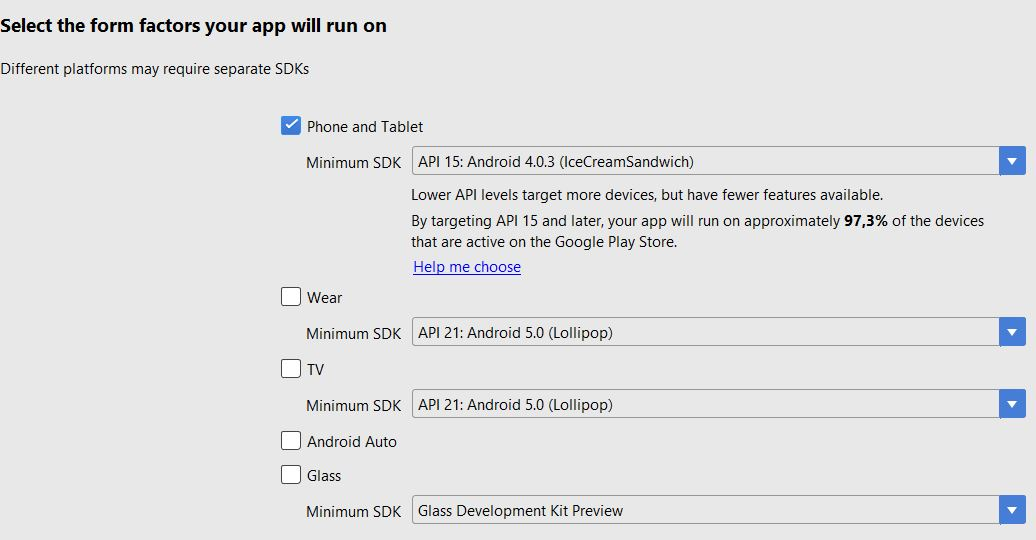
\includegraphics[width=1.0 \textwidth]{images/MinMaxVers}
	\caption{Version}\label{Fig:min-max Version}
\end{figure}



\clearpage % DO NOT REMOVE
\lfoot{Autor: Who?}
\subsubsection{Gängige Programmiersprachen}
\label{subsec:websprachen}

Lorem ipsum dolor sit amet, consectetur adipisicing elit, sed do eiusmod
tempor incididunt ut labore et dolore magna aliqua. Ut enim ad minim veniam,
quis nostrud exercitation ullamco laboris nisi ut aliquip ex ea commodo
consequat. Duis aute irure dolor in reprehenderit in voluptate velit esse
cillum dolore eu fugiat nulla pariatur. Excepteur sint occaecat cupidatat non
proident, sunt in culpa qui officia deserunt mollit anim id est laborum.

\clearpage % DO NOT REMOVE